\chapter{Introduzione}
\section{Prefazione}
Questa tesi consiste nella riproduzione e nello studio di \textit{sketch-rnn} \cite{sketchrnn}, una rete neurale in grado di generare disegni di semplici oggetti, composti da sequenze di tratti, appresi da un dataset di disegni creati da esseri umani. Il dataset è costantemente ampliato tramite \textit{Quick Draw!} \cite{quickdraw}, un gioco online in cui agli utenti viene chiesto di disegnare alcuni oggetti entro 20 secondi, che al momento della stesura di questa tesi costituisce la più vasta collezione di disegni al mondo. In questo lavoro viene proposta un'implementazione in \textit{Keras} \cite{keras}, un framework che a sua volta poggia su \textit{tensorflow} \cite{tensorflow}, che è la libreria utilizzata per il lavoro originale.
\begin{figure}[h]
	\centering
	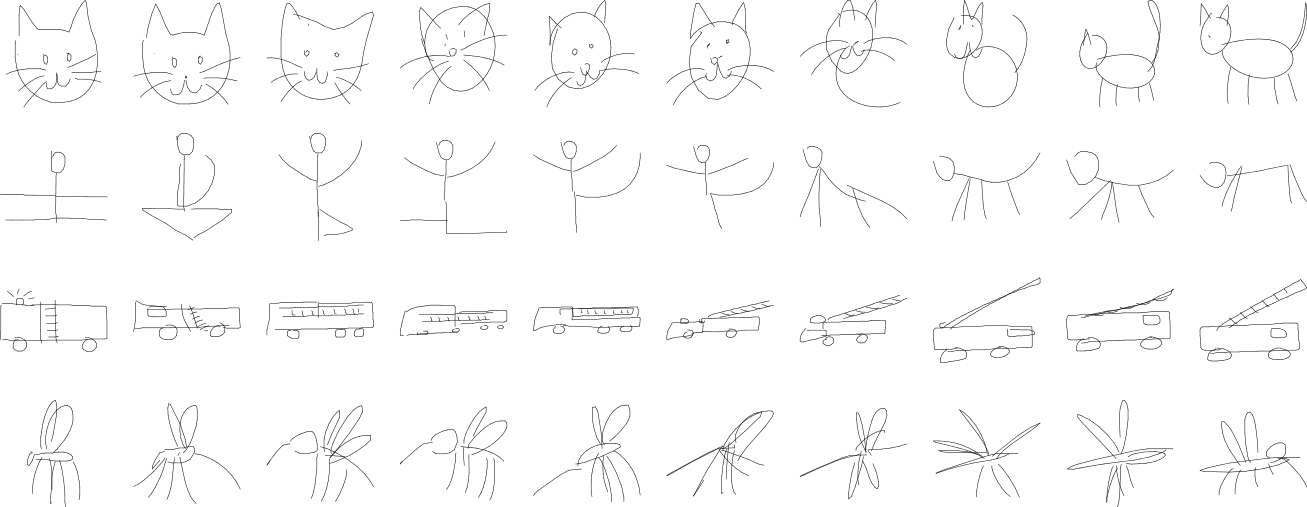
\includegraphics[width=\linewidth]{img/sketch_rnn_latent.png}
	\caption{Interpolazioni nello spazio di latenza di immagini vettoriali generate dal modello.}
	\label{fig:1.1}
\end{figure}
\section{Stato dell'arte}
Negli ultimi anni la generazione di immagini attraverso l'uso di reti neurali ha avuto ampia diffusione, fra i modelli più importanti possiamo citare \textit{Generative Adversarial Networks (GANs)} \cite{GAN}, \textit{Variational Inference (VI)} \cite{VI} e \textit{Autoregressive Density Estimation (AR)}. \cite{AR} Il limite della maggior parte di questi algoritmi è che lavorano con immagini in pixel a bassa risoluzione, a differenza degli esseri umani che, piuttosto che vedere il mondo come una griglia di pixel, astraggono concetti per rappresentare ciò che osservano. Allo stesso modo degli esseri umani, che fin da piccoli imparano a riportare i concetti appresi attraverso una sequenza di tratti su un foglio, questo modello generativo apprende da, e produce, immagini vettoriali.

L'obbiettivo è di addestrare una macchina a riprodurre ed astrarre concetti, in maniera analoga a come farebbe un essere umano. Ciò può avere numerose applicazioni in campo didattico come artistico, ad esempio assistendo il processo creativo, così come l'analisi della rappresentazione prodotta può offrire spunti di ricerca.
\section{Lavori correlati}

\section{Reti neurali}
Per spiegare le reti neurali e il Deep Learning si possono usare diversi approcci: uno consiste nel seguire il corso storico, introducendo il concetto di \textit{Percettrone}, passando ai Percettroni Multi-Strato ed ai primi metodi di ottimizzazione che furono applicati a questi modelli. Un altro approccio consiste nel partire da un punto di vista stocastico, definendo una regressione logistica che implica in modo naturale la minimizzazione di una \textit{loss function}. Ciò permette la definizione del concetto stesso di loss function e di come modificare dei parametri per ottenere una soluzione migliore, ciò si ricollega perfettamente al concetto di Percettrone Multi-Strato come classificatore di una regressione logistica.

Da qui in poi verrà proposta la spiegazione di alcuni modelli fondamentali del Deep Learning, che saranno considerati come "mattoni" costitutivi del modello studiato in questo progetto. Ciò aiuterà a comprendere agevolmente l'implementazione realizzata nel codice, seguendo un punto di vista coerente con le piattaforme più diffuse.
\section{Reti densamente connesse} % (fold)
\label{sec:reti_densamente_connesse}
Un neurone artificiale consiste in una funzione matematica che costituisce l'unità computazionale di base di una rete neurale artificiale.
\begin{figure}[h]
	\centering
	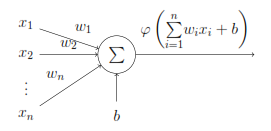
\includegraphics{img/artificial_neuron.png}
	\caption{Rappresentazione di un neurone artificiale.}
	\label{fig:1.2}
\end{figure}
Come si nota dalla figura \ref{fig:1.2} il neurone artificiale riceve \emph{n} input pesati $(w_1x_1,...,w_nx_n)$ e un bias \emph{b}. Successivamente li somma e applica una funzione non lineare nota come \textit{activation function} $\varphi$ per generare l'output. In sostanza calcolare l'output di un singolo neurone corrisponde a formare una combinazione lineare dei suoi input pesati e poi passarla ad una funzione di attivazione.

Per ragioni storiche, nel caso particolare in cui la funzione di attivazione consiste di una funzione con una soglia lineare (e output binario), il neurone è detto \textit{Percettrone}.

Da qui in poi, quando ci riferiremo ad un \textit{layer} di una rete neurale staremo parlando di un raggruppamento di neuroni che formano, nello specifico, una colonna nel grafo della figura \ref{fig:1.2}, ovvero neuroni che si trovano allo stesso livello di profondità nella rete. Inoltre, ogni layer che si trova fra quello di input e quello di output verrà chiamato \textit{hidden layer}.

Come detto in precedenza, un Percettrone Multi-Strato (MLP da Multi-Layer Perceptron) può essere visto come un classificatore a regressione logistica dove l'input è trasformato utilizzando una trasformazione non lineare appresa $h(\textbf{x})$ che costituisce l'hidden layer della nostra rete neurale (come in figura \ref{fig:1.2}). Questa trasformazione proietta l'input in uno spazio dove diventa linearmente separabile.

Questa computazione eseguita da una rete neurale multi-Strato, con un singolo hidden layer con una funzione di attivazione non lineare per elementi $\varphi_i$ sul vettore di input \textbf{x} e l'hidden output può essere scritta, in forma matriciale, come $\boldsymbol{y} = \varphi_2(W_2\varphi_1(W_1\boldsymbol{x} + \boldsymbol{b_1}) + \boldsymbol{b_2})$ dove $W_i, \boldsymbol{b_i}$ sono la matrice dei pesi e il vettore del bias dell'\textit{i}-esimo layer.

\begin{figure}[h]
	\centering
	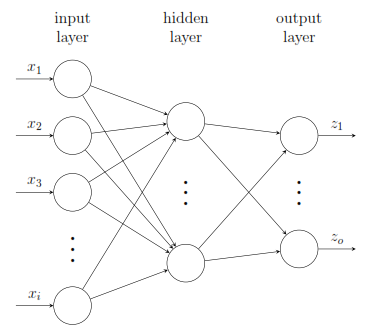
\includegraphics{img/MLN.png}
	\caption{Rappresentazione di un modello Multi-Strato.}
	\label{fig:1.3}
\end{figure}

Seguendo il teorema di approssimazione universale \cite{approx} possiamo affermare che una rete neurale con un singolo hidden layer contenente un numero finito di neuroni (ovvero un MLP) è abbastanza per approssimare qualunque funzione continua su un sottoinsieme compatto di $\mathbb{R}^n$.

Alcuni sinonimi rilevanti utilizzati al posto di reti neurali Multi-Strato 
sono \textit{dense layers}, \textit{fully-connected layers} o, meno diffuso, \textit{inner product layers}.
% section reti_densamente_connesse (end)
\section{Reti ricorrenti}
\begin{figure}[h]
	\centering
	\includegraphics{img/rnn.png}
	\caption{Una semplice RNN (Recurrent Neural Network).}
	\label{fig:1.4}
\end{figure}
Il cervello umano, nello specifico il lobo frontale, è in grado di elaborare conseguenze future risultanti da azioni nel presente, è in grado di selezionare fra buone e cattive azioni (o fra migliori e ideali) e può determinare somiglianze e differenze fra oggetti ed eventi.

Molti problemi richiedono, per essere risolti, di un certo grado di conoscenza pregressa. Un esempio può riguardare le variazioni della luce di un semaforo: se, per esempio, osserviamo che nel momento attuale la luce accesa è quella gialla, il nostro scopo sarebbe quello di sapere quale sarà la prossima ad accendersi. Le diverse posizioni delle luci in un semaforo sono irrilevanti: ciò che ci interessa è sapere quale colore apparirà, sapendo che quello appena apparso è il giallo. Nella maggior parte delle città sappiamo che la risposta sarebbe che il prossimo sarà il rosso. Per rispondere a questa domanda è venuta in nostro aiuto la nostra esperienza ma se provassimo a risolvere il problema utilizzando una rete neurale come quella proposta in precedenza non otterremmo una risposta soddisfacente. Ciò accade perché la soluzione presenta una dipendenza temporale, che corrisponde al metodo attraverso cui un essere umano apprende a risolvere problemi: analizzando sequenze di eventi.

Per trovare una soluzione a questo problema, com'è uso nel campo dell'Intelligenza Artificiale, viene tratta nuovamente ispirazione dai modelli basati sui principi biologici per elaborare una classe di reti neurali artificiali, in cui le connessioni fra le unità formano un ciclo orientato, dette Reti Neurali Ricorrenti (RNN da Recurrent Neural Networks, Fig. \ref{fig:1.4}). Queste connessioni creano uno stato interno della rete che le permette di esibire un comportamento dinamico nel tempo.


\subsection{Dipendenze a lungo termine} % (fold)
\label{sub:dipendenze_a_lungo_termine}

% subsection dipendenze_a_lungo_termine (end)
\subsection{Long Short Term Memory}
\subsection{Reti bidirezionali}
\section{Reti autoregressive}
\section{Autoencoder}
\subsection{Variational Autoencoder}
\section{MDN}